\section{Angriffe}
Im Rahmen dieser Ausarbeitung wollen wir uns auf die Ermittlung des \textit{Pre-shared Keys} (\textit{PSK}) als Angriffsziel und auf den Angriffsvektor des Brechens mitgeschnittener Handshakes durch Exploration des Schlüsselraumes (Bruteforce) beschränken.

Tatsächlich gibt es nach dem bekannten Stand der Forschung keine Schwachstellen im Protokoll von WPA2-PSK, die es einem, nicht der Nutzergruppe angehörenden, Angreifer ermöglichen würden, die Kommunikation zu entschlüsseln. Es gibt bspw. eine Schwachstelle (\enquote{Hole 196}), die die Ermittlung des PTKs anderer Teilnehmer ermöglicht -- allerdings muss dem Angreifer hierfür der PSK bekannt sein, was die praktische Relevanz des Angriffes drastisch reduziert.

Aufgrund der Aufmerksamkeit, der sich dieses Thema unter Netzwerkexperten und Kryptologen in der Vergangenheit erfreute, ist nicht damit zu rechnen, dass in dem Verfahren noch grundlegende Schwachstellen gefunden werden. 

Da die Sicherheit eines solches Verfahrens jedoch von mindestens drei Dingen abhängt -- der Sicherheit des Protokolls sowie der kryptografischen Primitiven, der fehlerfreien Implementierung und auch der Wahl eines guten Geheimnisses -- reicht dies allein nicht aus. 
So liegt die Wahl des Geheimnisses (in diesem Fall des Netzwerkschlüssels) meist in der Hand des nicht zwingend sachverständigen Endnutzers. 
So kann ein schlecht gewähltes Passwort oftmals durch einen durchdachten Wörterbuchangriff in realistischer Zeit gebrochen werden, ohne das Protokoll als solches angreifen zu müssen.\\

Eine weitere Spielwiese sind Social-Engineering-Angriffe, die auf Unwissenheit, Unaufmerksamkeit und Leichtgläubigkeit der Nutzer setzen. 
Durch die nachfolgend beschriebene \enquote{Auskunftsfreudigkeit} der meisten Endgeräte hinsichtlich ihrer bekannten Netzwerken ergeben sich für Tools dieser Kategorie Möglichkeiten ihre Angriffe plausibel und für die meisten Nutzer authentisch wirkend durchzuführen.
So strahlt zum Beispiel das Tool \textit{wifiphisher} über einen geeigneten Netzwerk-Adapter ein offenes Netzwerk mit beliebiger SSID aus und präsentiert sich verbundenen Nutzern je nach System verschiedene, teils täuschend echt aussehende Dialoge zur Eingabe des Netzwerkschlüssels. 
Um einen Nutzer in das eigene Netzwerk zu bringen nutzt das Tool den später beschriebenen Deauth-Angriff. 

\textit{Fluxion} prüft die vom Benutzer getätigten Eingaben zusätzlich gegen einen mitgeschnittenen Handshake ab und kann sich so dem Benutzer gegenüber authentisch Verhalten und Falscheingaben erkennen. 
Dieser und weitere Angriffe, wie sie beispielsweise in~\cite{caneill2010attacks} beschrieben sind, sollen in dieser Ausarbeitung jedoch nicht weiter betrachtet werden, da ihr Ansatz ein grundlegend anderer ist.\\

\subsection{Erfassen eines WPA2-Handshakes}
Bei Bruteforce-Angriffen unterteilt sich die Ermittlung des Netzwerkschlüssels (PSK) in zwei elementare Schritte: 
\begin{enumerate}
	\item Die Erfassung eines WPA2-PSK-Handshakes während der Authentifizierungsphase zwischen Client und AP
	\item Die nachgelagerte Suche nach einem Schlüssel, der zu einem gleichen Hashwert führt
\end{enumerate}
%TODO: Finde die Formulierung von dir oben schon ausreichend, außerdem ist der Footnote Bereich sonst zu groß
%\footnote{Theoretisch können auch mehrere Schlüsselkanditaten zu einer Hashkollision führen. Aufgrund der Längenbeschränkung von WPA2-Schlüsseln und der Güte der eingesetzten Hash-Verfahren hinsichtlich schwacher Kollisionsresistenz ist dies jedoch äußerst unwahrscheinlich und in der Praxis nicht von Belang.} 
Die vermutlich subtilste Methode zur Erlangung eines Handshakes, die dem Angreifer zur Verfügung steht, ist die passive Überwachung des Netzwerkverkehrs und abzuwarten, bis sich ein Client gegenüber einem AP im gewünschten Netzwerk authentifiziert. 
Abhängig von der Netzwerkinfrastruktur und des Nutzungsverhaltens des Clients kann dies jedoch viel Zeit in Anspruch nehmen.
Da dies für einen gezielten Angriff nicht zielführend erscheint werden nachfolgend zwei Angriffe beschrieben, die durch aktives Eingreifen in den Netzwerkverkehr die Authentifizierung des Clients forcieren.

\subsubsection{Deauth-Angriff}\label{subs:deauthentication-attack}
Wie in Kapitel~\ref{sec:grundlagen} bereits beschrieben definiert IEEE 802.11 neben Datenframes unter anderem auch Managementframes, die der Verwaltung des Netzwerkes dienen und weder verschlüsselt noch anderweitig authentifiziert auf dem exponierten Übertragungsmedium versendet werden.

Dies hat zur Folge, dass ein Angreifer Managementframes erzeugen und im Netzwerk unter einem gefälschten Absender an beliebige Teilnehmer verteilen kann.
So auch Deauthentication-Frames, mit denen ein Access-Point die erneute Authentifizierung vor einer weiteren Nutzung erzwingen kann. Der Idee ist nun sehr simpel: Der Angreifer kennt sein Opfer, gaukelt diesem durch gefälschte\footnote{In unseren Versuchen hat sich gezeigt, dass es meistens mehrerer Deauthentication-Pakete bedurfte, um den Client tatsächlich zu einem kurzzeitigen Verlassen des Netzwerkes zu bewegen. Die Wahl der Anzahl hat sich hierbei als Gratwanderung herausgestellt: werden zu wenig Pakete versendet führt der Client keine erneute Authentifizierung durch -- werden jedoch zu viele Pakete versendet, so konnten wir beobachten wie das Endgerät sich mit einem eigentlich niedriger priorisiertem Netzwerk verbunden hat, da ihm einer erneuter Verbindungsaufbau anscheinend nicht möglich erschien. Ein Wert von 20 hat sich in unseren Versuchen als zielführend erwiesen.} Deauthentication-Frames die Deauthentifizierung durch den AP vor um anschließend den provozierten Handshake mitschneiden zu können.
Die Felder des entsprechenden Deauthentication-Frame werden dabei wie folgt gesetzt:
\begin{itemize}
	\item als Zieladresse (DA) die MAC-Adresse des Clients
	\item als Quelladresse (SA) die MAC-Adresse des Access-Points
	\item als BSSID die MAC-Adresse des AP mit dem der Client kommuniziert
	\item ein beliebiger Reason-Code, bspw. \enquote{1} für \enquote{Unspecified Reason} \cite[S. 442]{ieee802.11}
\end{itemize}
Abbildung~\ref{fig:deauth-attack} zeigt ein solches Deauthentication-Frame sowie die vom Angreifer zu modifizierenden Felder.

\begin{figure}[ht]
	\centering
	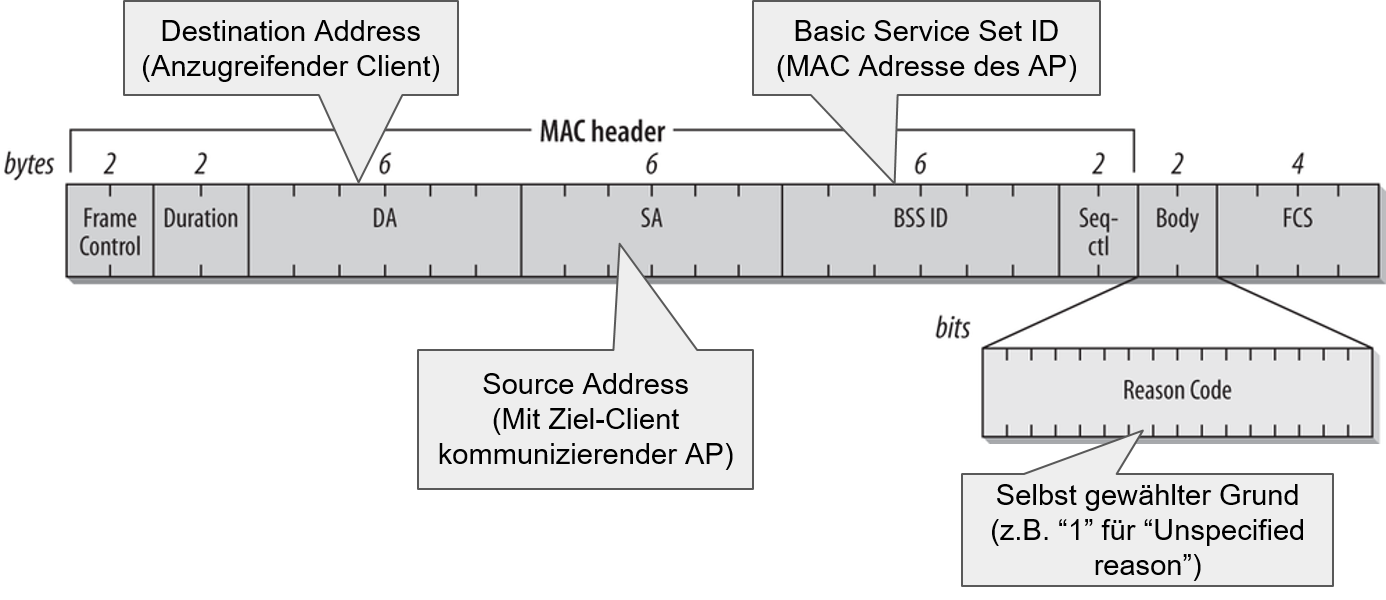
\includegraphics[width=0.95\textwidth]{graphics/deauth-attack}
	\caption[Deauthentication-Frame]{Für einen Deauth-Angriff müssen lediglich die MAC-Adressen des AP und des Clients bekannt sein.}
	% TODO Wo stammt die Grafik her? Quelle
	\label{fig:deauth-attack}
\end{figure}

Gemäß Spezifikation entspricht in Netzwerken, welche eine Authentifizierung erzwingen, eine Deauthentifizierung einer Disassozation (durch ein Disassociation-Frame herbeigeführte Verbindungsaufhebung)\footcite[S. 74, S. 442]{ieee802.11}. In einen einem Versuch gegen ein mit \textit{macOS 10.12.4} betriebenes Gerät konnten wir zeigen, dass -- auch wenn der Name es nicht suggeriert -- die Verwendung von Disassociation-Frames für diesen Angriff ebenfalls geeignet ist.

\paragraph{Durchführung}
Zur Durchführung des Deauth-Angriffs müssen zwei Bedingungen erfüllt sein: 
\begin{itemize}
	\item der Angreifer ist in Reichweite des Clients
	\item der Client ist mit einem Access-Points des Zielnetzwerks verbunden 
\end{itemize}
Zunächst versetzt der Angreifer sein Netzwerkinterface (z.B. \texttt{wlan0}) in den Monitor-Mode und beendet störende Hintergrundprozesse:
\texttt{airmon-ng check kill}\\
\texttt{airmon-ng start <Interface>}\\
Dies ermöglicht das Überwachen des Netzwerkverkehrs und das aussenden eigens erstellter Frames.
Um potentielle Handshakes und andere Pakete aufzuzeichnen verwendet der Angreifer \texttt{airodump-ng}:
\texttt{airodump-ng -c <Channel> --bssid <AP-MAC> -w <Dateiname> <Interface>}
Das Flag \texttt{--bssid} ist dabei optional.
Es verhindert, dass Pakete von anderen Access-Points aufgezeichnet werden und kann somit die nachträgliche Analyse erleichtern.
Sind die MAC-Adresse des Clients und des Access-Points bekannt startet der Angreifer mit Hilfe von \texttt{aireplay-ng} den Deauth-Angriff: 
\texttt{aireplay-ng -0 <Anzahl> -a <AP-MAC> -c <Client-MAC> <Interface>}
Das Flag \texttt{-0} kennzeichnet den Deauth-Angriff.
Via \texttt{<Anzahl>} kann spezifiziert werden, wie viele Deauthentication-Frames an das Ziel gesendet werden.
Ein Nachteil dieses Ansatzes ist, dass \texttt{aireplay-ng} mit dem Aussenden der Deauthentication-Frames wartet bis es einen Beacon-Frame des Access-Points erhalten hat.
Alternativ kann die Deauthentifikation \enquote{manuell} mithilfe von \texttt{Scapy} durchgeführt werden:
\texttt{Scapy Script hier}
Nach dem Angriff stoppen wir die eingangs gestartete Netzwerkaufzeichung von \texttt{airodump-ng} und analysieren den Dump mithilfe eines geeigneten Tools, zum Beispiel \texttt{Pyrit}:
\texttt{pyrit -r <Dump-Name> -b <AP-MAC> analyze}
Wurde die MAC-Adresse des Access-Points nicht beim Aufzeichnen des Verkehrs spezifiziert sollte sie nun mit dem Flag \texttt{-b} festgelegt werden.
Andernfalls wird \texttt{Pyrit} für eventuell weitere aufgezeichnete Handshakes von anderen Netzwerken mit einer positive Rückmeldung antworten.

\subsubsection{\enquote{Evil-Twin}-Angriff}\label{subs:evil-twin-attack}
Ein Nachteil des Deauth-Angriffs ist, dass sowohl der Client als auch der Access-Point in Reichweite des Angreifers sein müssen (on-site) um den Handshake zwischen beiden abfangen zu können.
Um den PSK eines WPA2-Netzwerks zu Bruteforcen ist jedoch kein vollständiger Handshake notwendig.
Den Angreifer benötigt lediglich folgende Informationen:
\begin{itemize}
	\item SSID des Netzwerkes 
	\item MAC-Adressen der Handshaketeilnehmer
	\item ANonce aus Schritt 1
	\item SNonce inklusive MIC aus Schritt 2
\end{itemize}
Die Parameter, die vom Access-Point übermittelt werden, unterliegen keinerlei Schutz und werden nicht auf Authentizität geprüft.
Der Angreifer kann demnach die ANonce und MAC-Adresse beliebig wählen und den Handshake bis zu Schritt zwei durchführen.
Um die übrigen Parameter zu erhalten (SNonce inklusive MIC) muss der Angreifer dem Client ein authentisches, ihm bekanntes Netzwerk vortäuschen.
Dafür öffnet der Angreifer einen eigenen Access-Point mit der SSID des Zielnetzwerks und passender Konfiguration: den sogenannten Evil-Twin.
Die Konfiguration entspricht einer der folgenden Möglichkeiten: Open, WEP, WPA-PSK, WPA-Enterprise, WPA2-PSK, WPA2-Enterprise.
Der Angreifer rät nun die richtige Konfiguration oder öffnet alternativ mehrere Access-Points die alle Möglichkeiten abdecken.
Ist das Zielnetzwerk bekannt (und somit auch die SSID), so ist der Evil-Twin einsatzbereit und funktionsfähig.

Oft ist jedoch ein konkreter Client Ziel des Angriffs (zum Beispiel Man in the Middle) und die dem Client bekannten Netzwerke sind dem Angreifer verborgen.
In diesem Fall bedient sich der Angreifer der in Sektion~\ref{Einleitungoderso} beschriebenen Probe-Requests, die vom Client kontinuierlich gesendet werden.
Aus diesen kann der Angreifer die SSIDs auslesen und gegebenenfalls mehrere Access-Points öffnen.
Die gesammelten Handshakes dienen als Grundlage für einen Angriff in die Breite: Anstelle komplexere Passwörter als Kandidaten gewählt werden wird nach der \enquote{lowest hanging fruit}, also dem Netzwerk mit dem schwächsten PSK gesucht.

\paragraph{Durchführung}
Für den Evil-Twin Angriff bietet Aircrack-ng zwei mögliche Herangehensweisen, die folgend näher beleuchtet werden sollen.
Zunächst muss, wie beim Deauth-Angriff bereits beschrieben, das Netzwerkinterface in den Monitor-Mode versetzt werden.
Weiß der Angreifer im Vorfeld für welche SSID er den Evil-Twin öffnen möchte, so kann er dafür den folgenden Befehl verwenden:
\\\texttt{airbase-ng start --essid <SSID> -Z 4 -F <Dateiname> <interface>}\\
Durch das Flag \texttt{-Z 4} wird sich der Evil-Twin als WPA2-PSK geschützter Access-Point ausgeben.
Mithilfe des Flags \texttt{-w} wird der Netzwerkverkehr zwischen dem Evil-Twin und den Clients mitgeschnitten.
Versucht sich ein Client nun mit dem Evil-Twin zu verbinden wird der Handshake bis zu Schritt zwei durchgeführt, mitgeschnitten und in dem Dump \texttt{<Dateiname>} gespeichert.
Danach wird die Authentifikation im Schritt 3 abgebrochen.
Dies äußert sich beim Client in Form einer Fehlermeldung wie zum Beispiel: \enquote{Fehler bei der Authentifizierung}.
Es können beliebig viele Evil-Twins auf dem selben Interface geöffnet werden. 
Dies ist nützlich, wenn mehrere Handshakes eines Clients von verschiedenen Netzwerken abgefangen werden sollen oder die Sicherheitskonfiguration eines konkreten Netzwerks unbekannt ist.
In letzterem Fall werden mehrere Evil-Twins mit gleicher SSID, aber unterschiedlichen Flags geöffnet (z.B.\texttt{-Z 4} für WPA-PSK). %TODO: Commands prüfen


Besitzt der Angreifer hingegen keine bekannten SSIDs seines Ziels, so kann er das \texttt{-P} Flag unter Airbase verwenden ohne eine SSID anzugeben:
\\\texttt{airbase-ng start -P -Z 4 <interface>}\\
Airbase wird nun auf dem ausgewählten Interface Probe-Requests von Clients mitlesen und auswerten um automatisch Evil-Twins mit der vom Angreifer spezifizierten Sicherheitskonfiguration zu erzeugen.
Wir empfehlen gleichzeitig einen \texttt{airodump-ng} Prozess zu starten, der den Verkehr des Evil-Twins separat aufzeichnet.
Dies hat den Hintergrund, dass die Aufzeichnung von \texttt{airbase-ng} ohne spezifizierte SSID via \texttt{--essid} Flag den Wert \texttt{default} als Netzwerknamen verwendet anstelle des Wertes aus der Probe-Requests.
Ohne gültige SSID werden diese Handshakes jedoch unbrauchbar, da diese in die Berechnung des PMK mit einfließt.

\subsection{Handshake Bruteforcing}
Nachdem die notwendigen Schritte des Handshakes erfolgreich abgefangen wurden kann der Angreifer den PSK offline brechen.
Dafür spielt er die Schritte, die Client und Access-Point während dem Handshake durchführen, lokal nach und wählt dabei in jedem Versuch einen neuen Passwortkandidaten.
Folgende Schritte sind dafür nötig:
\begin{enumerate}
	\item Berechne $PMK = PBKDF2(SSID, PSK, 4096)$
	\item Verwende die aufgezeichneten Noncen und berechne damit \\$PTK = PRF(Client-MAC, Access-Point-MAC, SNonce, ANonce, PMK)$\footnote{Im Standard wird die entsprechende Pseudo-Zufalls-Funktion (PRF) definiert.}
	\item Bilde den MIC über den PTK Kandidaten und vergleiche ihn mit dem aufgezeichneten
	\begin{enumerate}
		\item MICs sind ungleich: gehe zu Schritt 1
		\item MICs sind gleich: Handshake erfolgreich gebrochen
	\end{enumerate}
\end{enumerate}
Den Großteil des Rechenaufwands benötigt das bilden des PMKs in Schritt 1 über 4096 Runden PBKDF2.
Des weiteren können nur selten PMK-Listen vorab generiert werden, da der PMK auch von der SSID des Netzwerkes abhängig ist.

\paragraph{Durchführung}
Es existieren verschiedenste Tools und Online-Services zum brechen von WPA2-PSK Handshakes.
Wir werden folgend ausschließlich das Vorgehen mit \texttt{aircrack-ng} erläutern, jedoch weitere nützliche Tools sowie ihre Vorteile erwähnen.

\texttt{Aircrack-ng} erfordert zum Brechen die ersten zwei Schritte des WPA2-PSK Handshakes gespeichert in einem Capture-File (z.B. .cap).
Die dabei übertragenen Pakete enthalten die übrigen, für den Angriff nötigen Parameter wie MAC-Adressen beider Teilnehmer und SSID des Netzwerkes.
Weiterhin ist eine Passwortliste erforderlich die PSK Kandidaten enthält, welche \texttt{aircrack-ng} für den aufgezeichneten Handshake prüfen soll.
Sind alle Vorbedingungen erfüllt, können wir den Angriff durchführen:
\\\texttt{aircrack-ng -w <Passwortliste> -b <AP-MAC> <Capture>}\\
Sofern während der Aufzeichnung sichergestellt wurde, dass ausschließlich Verkehr des anzugreifenden Access-Points aufgezeichnet wurde kann das Flag \texttt{-b} verworfen werden.
\texttt{Aircrack-ng} wird nun pro PSK-Kandidat in 4096 Runden PBKDF2 den dazugehörige PMK-Kandidaten berechnen, daraus den PTK ableiten und den entsprechenden MIC bilden.
Wird ein MIC gebildet, der mit dem aufgezeichneten MIC übereinstimmt, wurde eine Kollision erzeugt und das dazugehörige Passwort wird ausgegeben.

Es existieren weitere Tools zum Cracken von WPA2-PSK Handshakes, die mehr Funktionalität zu Kosten erhöhter Komplexität bieten.
So bietet \texttt{Pyrit} dem Nutzer die Möglichkeit Datenbanken mit vorberechneten PMKs zu importieren oder eigens aus Passwortlisten zu erstellen.
\texttt{Hashcat} und \texttt{oclHashcat} hingegen werben mit hoher Performance und einer breiten Masse an Algorithmen.
%Angriff in die Breite ist ein Thema, welches Erik interessiert. Einfaches Einsammeln vieler Handshakes und Vergleichen mit einem einmal berechneten Hash nicht möglich, da Hash eine Nonce enthält und somit Handshake auch bei gleicher Passphrase verschiedene Hashes enthält. Allerdings sind die "verschiedenen Stufen des Bruteforcens" (damit meine ich: Kontextabhängige Passwörter (bspw. (modifizierte) SSID) , Wörterbuch häufiger Passwörter, Kombinieren verschiedener Wörterbucheinträge bzw. Kombinieren mit Zahlen, tatsächliche, systematische Exploration des Suchraumes) unterschiedlich effizient. So dürfte die Wahrscheinlichkeit, dass ein Passwort einem Wort X aus einem Wörterbuch entspricht deutlich höher sein, als dass es einer gänzlich zufälligen Ziffern-/Zeichenfolge y entspricht. Es sollte daher auf die Idee eingegangen werde, sich auf Wörterbuchangriffe zu beschränken, diese jedoch auf eine Vielzahl von Handshakes (ausgehend von einem Endgerät) loszulassen. Üblicherweise dürften die meisten Nutzer sich in der Vergangenheit auch mit WLANs mit schlechten Passwörtern verbunden haben, daher wird nach der "lowest hanging fruit" gesucht. Soll gezielt die Kommunikation mit einem Netzwerk belauscht werden ist dies nicht von Nutzen, für eine Vielzahl anderer Angriffe jedoch durchaus, bspw. für einen MITM-Angriff via Evil-Twin, DNS-Hijacking, ARP-Spoofing etc..